\documentclass[11pt]{article}

\usepackage[a4paper,margin=0.8in]{geometry}
\usepackage{amsfonts}
\usepackage{amsmath}
\usepackage{amsthm}
\usepackage[linesnumbered,ruled,vlined]{algorithm2e}
\usepackage{cleveref}
\usepackage{ifthen}
\usepackage{rotating}
\usepackage{tikz}
\usepackage{caption}
\usepackage{graphicx}

\SetKwInput{KwInput}{Input}                % Set the Input
\SetKwInput{KwOutput}{Output}   

\begin{document}
\author{Marco Milanta}
\title{Graded Homework 2, exercise 2}
\maketitle
% actually edit those files and create new sections if you need more. 

%% Special characters for number sets.
\newcommand{\N}{\mathbb{N}}


\newcommand{\R}{\mathbb{R}}
\newcommand{\E}{\mathbb{E}}

%% Vectors and sets.
\newcommand{\set}[1]{\mathcal #1}
\newcommand{\mat}[1]{\mathbf #1}
\renewcommand{\vec}[1]{\mathbf #1}
\newcommand{\x}{\mathbf{x}}
\newcommand{\w}{\mathbf{w}}
\newcommand{\X}{\mathcal{X}}
\newcommand{\D}{\mathcal{D}}
\newcommand{\ke}{\mathbf{k}}
\newcommand{\K}{\mathbf{K}}
\newcommand{\A}{\mathbf{A}}
\newcommand{\Y}{\mathbf{Y}}
\newcommand{\Si}{\Sigma}
%\newcommand{\Pr}{\mathbb{P}}

%% Bold greek letters.
\newcommand{\lm}{\boldsymbol{\lambda}}
\newcommand{\tht}{\boldsymbol{\theta}}
\newcommand{\ph}{\boldsymbol{\phi}}
\newcommand{\omg}{\boldsymbol{\omega}}

%% Theorems
\newtheorem{observation}{Observation}
\section*{Minimizing Cost (25 points)}
Given a stream of $n$ elements $x_1, \cdots, x_n \in \{1,\cdots,n\}$ all distinct (i.e., the input is a permutation). We have to choose $x_i, x_j$ with $j\geq i$ on arrival, meaning that when an element arrives, we must immediately decide if we include it in one of the two elements. The cost function is given as $\frac{1}{x_j-x_i+1}$. We would like to minimize this cost. (Note that any sensible strategy will have $\frac{1}{x_j-x_i+1} < 1$ as we can choose $i=j=n$.)
\begin{enumerate}
    \item Find a deterministic algorithm that achieves competitive ratio at most $\sqrt{n}$.
    \item Show that any randomized algorithm has competitive ratio at least $\Omega(\sqrt{n})$
\end{enumerate}
\section*{Solutions}
\begin{enumerate}
    \item We propose the following algorithm. Note that we index arrays starting from 1.
    \begin{algorithm}[!ht]
        \SetKwProg{Def}{def}{:}{}
        \DontPrintSemicolon
        \KwInput{$X\in $ permutations of $\{1,\dots,n\}$}
        \KwOutput{$i,j, \frac{1}{x_j-x_i+1}$}
        $\mathtt{Seen} \gets [0,\dots,0] \in \mathbb{N}^n$\;
        $\mathtt{Missing} \gets [1,\dots,n] \in \mathbb{N}^n$\;
        $\mathtt{ChosenElements} \gets 0$\;
        $x_i \gets x_j \gets 0$\;
        \For{$k \in 1, \dots, n-1$}{
            \If{$\mathtt{ChosenElements} = 0$}{
                $\mathtt{Missing}[X[k]] \gets 0$\;
                $\mathtt{optFutu} \gets \max \;\mathtt{Missing}$\;
                \If{$(\mathtt{optFutu} - X[k] + 1)\geq \sqrt{n}$}{
                    $x_i \gets X[k]$\;
                    $i \gets k$\;
                    $\mathtt{ChosenElements} \gets 1$\;
                }
            }
            \ElseIf{$\mathtt{ChosenElements} = 1$}{
                \If{$X[k] = \max \; \mathtt{Missing}$}{
                    $x_j \gets X[k]$\;
                    $j \gets k$\;
                    $\mathtt{ChosenElements} \gets 2$
                }
            }
        }
        \If{$\mathtt{ChosenElements} = 0$}{
            $x_i \gets x_j \gets X[n]$\;
            $i \gets j \gets n$\;
        }
        return $i, j, \frac{1}{x_j-x_i+1}$\;
        \caption{Online algorithm}\label{a}
        \end{algorithm}
        \paragraph*{Legality of the algorithm.}
        Before analyzing the competitive ratio of this algorithm, I would like to notice that it has the correct structure. Notice these two facts:
        \begin{itemize}
            \item In the $k-$th iteration of the loop, we only look at $X[k]$. This means that our algorithm doesn't cheat by looking into the future. Finally, we look at the last element after the loop.
            \item $x_i$ and $x_j$ are assigned only once, always $x_i$ before $x_j$, and they are assigned to be $X[k]$ at the $k-$th iteration. Or, at latest, after the for loop. All of this is guaranteed by the counter $\mathtt{ChosenElements}$. This means that we are respecting the constraint "when an element arrives, we must immediately decide if we include it in one of the two elements".
            \item The algorithm iterates over the input elements, therefore is polynomial in $n$.
        \end{itemize}
        \paragraph*{Competitiveness of the algorithm.}
        Now we want to analyze the performance. To do so, let $\hat i, \hat j, \hat i \leq \hat j$ be an optimal solution that minimize $\frac{1}{x_{\hat j}-x_{\hat i}+1}$. We call $OPT$ the $\mathtt{cost}$ of the optimal algorithm. Notice that the optimal cost cannot go lower $\frac{1}{n}$, this is achieved when we manage to get $x_i = 1, x_j = n$.
        \begin{theorem}[Algorithm \ref{a} is $\sqrt{n}$-competitive] The algorithm \ref{a} is $\sqrt{n}$-competitive against the optimal solution. Or, formally, let $i, j, \mathtt{cost}$ be the output of the algorithm \ref{a}. Let $OPT$ be the maximal profit, then, for any input
            \begin{equation*}
                \mathtt{profit}\leq \sqrt{n} OPT.
            \end{equation*}
        \end{theorem}
        \begin{proof}
            We divide the proof in two parts depending on the behavior of the algorithm. 
            \paragraph*{Case 1:}(there is a $k \in {1,\dots,n-1}$ for which we enter the $\mathbf{if}$ at line $9$) Let for now $k$ be the iteration in which we enter the $\mathbf{if}$ at line $9$. One can notice that we will end up with a final cost of $\frac{1}{\mathtt{optFutu} - X[k] + 1}$. This is because we chose $x_i = X[k]$, and then we chose $x_j$ to be the maximal value among the remaining ones. We can safely find such value since we are keeping track of the missing ones $(\mathtt{optFutu})$. Once $\max \mathtt{Missing}$ will arrive, we pick it for $x_j$. 
            Notice that we cannot miss it since we are only looking at permutations as inputs. Hence, our algorithm has a cost of 
            \begin{equation*}
                \mathtt{cost} \frac{1}{x_j-x_i +1}=\frac{1}{\mathtt{optFutu} - X[k] + 1}.
            \end{equation*}
            Using this, we get that:
            \begin{equation*}
                \mathtt{cost} = \frac{1}{\mathtt{optFutu} - X[k] + 1} \stackrel{(i)}{\leq}\frac{1}{\sqrt{n}} =  \sqrt{n}\frac{1}{n}\ \stackrel{(ii)}{\leq} \sqrt{n}OPT.
            \end{equation*}
            Where $(i)$ follows from the fact that we enter the $\mathbf{if}$ at line $9$, and therefore $\mathtt{optFutu} - X[k] + 1 \geq \sqrt{n}$. $(ii)$ follows from the fact that minimum possible cost is $\frac{1}{n}$. In this scenario we have shown that the algorithm is $\sqrt{n}$ competitive.
            \paragraph*{Case 2:}(we never enter the $\mathbf{if}$ at line $9$) In this scenario, our algorithm picks $x_i = x_j = n$, and our $\mathtt{costs}$ will be $1$. We now want to show that $OPT \geq \frac{1}{\sqrt{n}}$. 
            
            To do so, we continue by contradiction. Assume that the optimal solution takes $\hat i \leq \hat j$ such that $OPT = \frac{1}{x_{\hat j}-x_{\hat i}+1} < \frac{1}{\sqrt{n}}$. This yields that 
            \begin{equation*}
                x_{\hat j}-x_{\hat i}+1 > \sqrt{n}.
            \end{equation*}
            Now we look at the behavior of our algorithm in this setting. Let's observe the moment when it gets to step $k = \hat i$. In this step $\mathtt{optFutu} = \max \mathtt{Missing} \geq x_{\hat j}$ (this is true since $\hat j > \hat i$, it's not equal, otherwise OPT cost would be 1). This yields that $\mathtt{optFutu} - X[\hat i] + 1 \geq x_{\hat j} -x_{\hat j} + 1 > \sqrt{n}$, which itself it yields that we enter the $\mathbf{if}$ at line $9$. This is however a contradiction. 

            From this we have that $OPT \geq \frac{1}{\sqrt{n}}$, and we get:
            \begin{equation*}
                \mathtt{cost} = 1 = \sqrt{n}\frac{1}{\sqrt{n}} \leq \sqrt{n}OPT.
            \end{equation*}
            \paragraph*{Conclusion:}We have shown that independently of which part of the algorithm triggers, we can guarantee that it outputs a $\sqrt{n}$-competitive solution
        \end{proof}
    \item Let $OPT(x)$ be the optimal $\mathtt{cost}$ achievable given $x\in \X$, where $\X$ is the space of permutation of $\{1,\dots,n\}$. Let's define a distribution over inputs $\mathcal{P}$ indexed by a discrete density $p:\X \to [0,1]$:
    \begin{equation}\label{Pdef}
        p(x) = \begin{cases}
            \frac{1}{2}& x = \bar{x}_1\\
            \frac{1}{2}& x = \bar{x}_2\\
            0 & \text{otherwise}
        \end{cases}
    \end{equation}
    Where $\bar x_1,\bar x_2$ are just aliases for
    \begin{align*}
        \bar x_1 &= \left\{n-1,n-2, \dots, 1 + n - \sqrt{n}, n, n -  \sqrt{n},  n - \sqrt{n} - 1, \dots, 1\right\}\\
        \bar x_2 &= \{n-1,n-2, \dots , 1, n\}.
    \end{align*}
    Notice that we are assuming that $\sqrt{n}$ is an integer (we don't generalize here, but we are sure that the idea generalizes as well). To visualize them better, look at figure below. 
    \begin{center}
        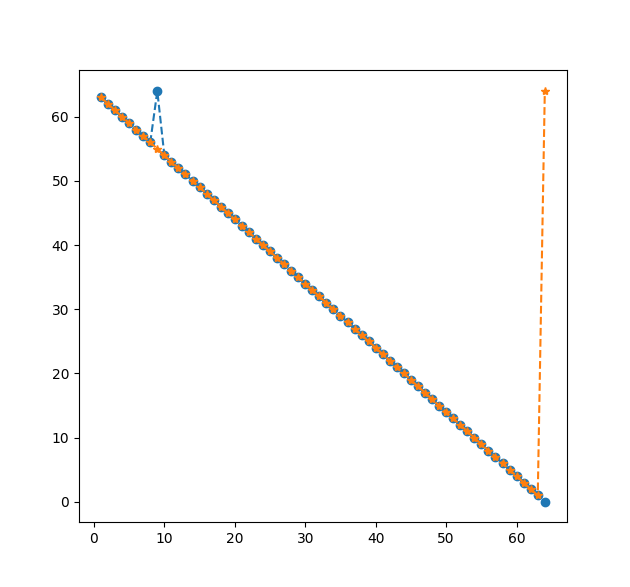
\includegraphics[scale=.5]{plot.png}
    \end{center}
    Where $\bar x_1$ is represented with blue dots and $\bar x_2$ with orange stars. In this plot $n = 64$.

    Now we state a key lemma that shows the importance of the chosen $\mathcal{P}$. 
    \begin{lemma}\label{lem1}[Best distribution] Given $x\sim \mathcal{P}$, any possible deterministic algorithm $\Alg$ has an expected competitive ratio of at least $\frac{1}{2}\left(\sqrt{n} + 1\right)$. Formally we have that,
    \begin{equation*}
        \E_{x \sim \mathcal{P}}\left[\frac{\Alg(x)}{OPT(x)}\right] \geq \frac{1}{2}\left(\sqrt{n} + 1\right)\qquad \text{for any $\Alg$ deterministic algorithm}
    \end{equation*}
    \end{lemma}
    \begin{proof}
        We start by defining two deterministic algorithms: $\Alg_1$ and $\Alg_2$. 
        \begin{itemize}
            \item $\Alg_1$ waits all the way to $1 + n - \sqrt{n}$, then buys $x_i = 1 + n - \sqrt{n}$. $\Alg_1$ then waits for $n$ to appear and then picks it (note that it will always appear). \item $\Alg_2$ commits and wait all the way to the second to last element, and then picks it. $\Alg_2$ then picks the last element if $n$ is the only missing element, and it buys the second to last again if the only missing element is $1$. 
        \end{itemize}
        \paragraph*{$\Alg_1$ and $\Alg_2$ competitive ratio:}
        looking at the behavior of the algorithms, and at how $\bar x_1$ and $\bar x_2$ are defined, we can compute the cost of the optimal algorithm, of $\Alg_1$ and of $\Alg_2$ on the inputs $\bar x_1$ and $\bar x_2$:
    \begin{align*}
        OPT(\bar x_1) &=\frac{1}{n - 1 - n - \sqrt{n} + 1}  = \frac{1}{\sqrt{n}}\\
        OPT(\bar x_2) &= \frac{1}{n - 1 + 1}= \frac{1}{n}\\
        \Alg_1(\bar x_1) &=\frac{1}{n - 1 - n - \sqrt{n} + 1}  = \frac{1}{\sqrt{n}}\\
        \Alg_1(\bar x_2) &= \frac{1}{n - 1 - n - \sqrt{n} + 1} = \frac{1}{\sqrt{n}}\\
        \Alg_2(\bar x_1) &= \frac{1}{n - 1 - (n - 1) + 1} = 1\\
        \Alg_2(\bar x_2) &=\frac{1}{n - 1 + 1}= \frac{1}{n}.
    \end{align*}

    Now we can compute:
    \begin{align*}
        \E _{x\sim \mathcal{P}}\left[\frac{\Alg_1(x)}{OPT(x)}\right] &=  p\left(\bar x_1\right)\frac{\Alg_1(\bar x_1)}{OPT(\bar x_1)}+ p\left(\bar x_2\right)\frac{\Alg_1(\bar x_2)}{OPT(\bar x_2)}\\
        &= \frac{1}{2}\left(\frac{\frac{1}{\sqrt{n}}}{\frac{1}{\sqrt{n}}}+ \frac{\frac{1}{\sqrt{n}}}{\frac{1}{n}}\right) = \frac{1}{2}\left(1 + \sqrt{n}\right)
    \end{align*}
    And we also do it for $\Alg_2$:
    \begin{align*}
        \E _{x\sim \mathcal{P}}\left[\frac{\Alg_2(x)}{OPT(x)}\right] &=  p\left(\bar x_1\right)\frac{\Alg_2(\bar x_1)}{OPT(\bar x_1)}+ p\left(\bar x_2\right)\frac{\Alg_2(\bar x_2)}{OPT(\bar x_2)}\\
        &= \frac{1}{2}\left(\frac{1}{\frac{1}{\sqrt{n}}}+ \frac{\frac{1}{{n}}}{\frac{1}{n}}\right) = \frac{1}{2}\left(\sqrt{n} + 1\right)
    \end{align*}
    \paragraph{Any other algorithm: } Now we want to show that the result doesn't only hold fore $\Alg_1$ and $\Alg_2$, but also for any other deterministic algorithm. For this we group all the possible algorithms in $2$ groups:
    \begin{itemize}
        \item \textbf{Group 1}: algorithms that pick as first element an element before $1 + n - \sqrt{n}$ both in $\bar x_1$ and $\bar x_2$
        \item \textbf{Group 2}: Every algorithm which is not in \textbf{Group 1}, and it's not $\Alg_1$ or $\Alg_2$.
    \end{itemize}
    First we show that any algorithm in \textbf{Group 1} costs more than $\Alg_1$ independently of the input $\bar x_1$ and $\bar x_2$. Let $\mathcal C$ be an algorithm in \textbf{Group 1}: it picks the first element $c_1$ before $1 + n - \sqrt{n}$, and then it picks $c_2$. This implies
    \begin{equation*}
        \mathcal C(\bar x _ 1) = \mathcal C(\bar x _ 2) = \frac{1}{c_2-c_1+1}  \stackrel{(i)}{<} \frac{1}{c_2 - (1 + n - \sqrt{n}) +1} \stackrel{(ii)}{\leq} \frac{1}{n - 1 - n + \sqrt{n} +1} = \frac{1}{\sqrt{n}}
    \end{equation*}
    Where the inequality $(i)$ holds since we $c_1$ is before $1 + n - \sqrt{n}$, and therefore $c_1 > 1 + n - \sqrt{n}$. $(ii)$ holds since $c_2 \leq n$. Notice that both in $\bar x_1$ and $\bar x_2$ the cost of $\mathcal{C}$ is more than $\frac{1}{\sqrt{n}} = \Alg_1(\bar x_1) =\Alg_1(\bar x_2)$. Therefore: 
    \begin{equation*}
        \E _{x\sim \mathcal{P}}\left[\frac{\mathcal{C}(x)}{OPT(x)}\right] \geq \E _{x\sim \mathcal{P}}\left[\frac{\Alg_1(x)}{OPT(x)}\right] \geq \frac{1}{2}(\sqrt{n} + 1).
    \end{equation*} This concludes the proof for \textbf{Group 1}.

    We now notice that all the algorithms in \textbf{Group 2} buy the first element after $1 + n - \sqrt{n}$. This is not trivial since in \textbf{Group 1} there are the algorithms that pick the first element before $1 + n - \sqrt{n}$ both in $\bar x_1$ and $\bar x_2$. What about the algorithms that depending on the input chose to pick either before or after $1 + n - \sqrt{n}$? Such algorithm cannot exist among deterministic ones, this is because the first elements before $1 + n - \sqrt{n}$ are exactly the same in $\bar x_1$ and $\bar x_2$, therefore, a deterministic algorithm that picks an element before $1 + n - \sqrt{n}$ will do it in both inputs, and vice versa, if it doesn't pick it before $1 + n - \sqrt{n}$ it will not do it in both inputs.

    Now, once we observed this, it is easy to notice that all algorithms in group to get a cost of at least $1$ on the input $\bar x_1$, this is because they "missed" the spike at $1 + n - \sqrt{n}$. 
    
    Now let $\mathcal {B}$ be our algorithm in \textbf{Group 2}. Let $c_1$ be the element $\mathcal {B}$ picks first on the input $\bar x_2$, and $c_2$ the other. $c_1>1$, otherwise the algorithm is $\Alg_2$, but \textbf{Group 2} doesn't contain $\Alg_2$. And, as before, $c_2\leq n$. This yields that the cost in input $\bar x_2$ is 
    \begin{equation*}
        \mathcal {B}(\bar x_2) = \frac{1}{c_2 - c_1 + 1} \geq  \frac{1}{n - c_1 + 1} > \frac{1}{n-1+1} = \frac{1}{n}.
    \end{equation*}
    Furthermore, from the observation before, we have $\mathcal{B}(\bar x_1) \geq 1$. Finally, we can observe that $\mathcal{B}$ does strictly worse than $\Alg_2$ both in $\bar x_1$ and $\bar x_2$. Therefore
    \begin{equation*}
        \E _{x\sim \mathcal{P}}\left[\frac{\mathcal{B}(x)}{OPT(x)}\right] \geq \E _{x\sim \mathcal{P}}\left[\frac{\Alg_2(x)}{OPT(x)}\right] \geq \frac{1}{2}(\sqrt{n} + 1).
    \end{equation*}
    Finally, this concludes the proof also for \textbf{Group 2}. It's easy to see that any algorithm is either $\Alg_1,\Alg_2$, inside \textbf{Group 1} or inside \textbf{Group 2}, hence we have concluded the proof.
    \end{proof}
    Now, the result simply follows from Yao's principle,
    \begin{equation*}
        \max_{x \in \X} \frac{\E_{\text{a}\sim \mathcal{A}}[a(x)]}{OPT(x)} \stackrel{(i)}{=} \max_{x \in \X} \E_{\text{a}\sim \mathcal{A}} \left[\frac{a(x)}{OPT(x)}\right] \stackrel{(ii)}{\geq} \min_{\Alg \in \text{det. algos}}\E_{x \sim \mathcal{P}}\left[\frac{\Alg(x)}{OPT(x)}\right] \stackrel{(iii)}{\geq} \frac{1}{2}(\sqrt{n} + 1) \in \Omega(\sqrt{n})
    \end{equation*}
    Where $(i)$ follows from linearity of expectation, $(ii)$ is a direct application of Yao's principle, and $(iii)$ follows from Lemma \ref{lem1}. 
    Being the first term of the last equation the competitive ratio of an arbitrary randomized algorithm $\mathcal A$, we have showed that it is in $\Omega\left(\sqrt{n}\right)$, and therefore, we have concluded the proof.
\end{enumerate}
\end{document}